\documentclass[12pt]{article}
\usepackage[T1]{fontenc}
%\usepackage[latin9]{inputenc}
\usepackage[utf8]{inputenc}
\usepackage[english]{babel}
\usepackage{amsmath}
\usepackage{amsfonts}
\usepackage{amssymb}
\usepackage{setspace}
\usepackage{rotating}
\usepackage{graphics}
\usepackage[round]{natbib}
%\usepackage{graphicx}
%\usepackage{float} 				%allows you to float images
\usepackage{latexsym}
\usepackage{bbding}
%\usepackage {moresize}
\usepackage{listings}
\usepackage{bbding}
\usepackage{blindtext}
\usepackage{hhline}
\usepackage{tikz}
\usetikzlibrary{trees}
%\usetikzlibrary{shapes,backgrounds}
%\usepackage{pgfplots}
%\usetikzlibrary{arrows}
\usepackage{enumitem}
\doublespacing
%\usepackage{geometry}
\usepackage{amsthm}
\usepackage{color}
%\usepackage{array,multirow}
%\usepackage{subcaption}
%\usepackage{pst-plot}
%	\psset{xunit=15mm}
%\geometry{verbose,tmargin=1in,bmargin=1in,lmargin=.5in,rmargin=.5in}
\setlength{\parskip}{\bigskipamount}
\setlength{\parindent}{0pt}
\usepackage{multicol}

\newenvironment{problem}[3][Problem]{\begin{trivlist}
\item[\hskip \labelsep {\bfseries #1}\hskip \labelsep {\bfseries #2.}]}{\end{trivlist}}

\title{Problem Set 2 \thanks{Problems 2,3,7,9,11}}
\author{Ian McGroarty \\
	Course Number: 625.641}
\date{June 25, 2019}

\begin{document}

\maketitle
\newpage
%%%%%%%%%%%%%%%%%%%%%%%%%%%%%%%%%%%%%%%%%%%%%%%%%%%%%%%%
%%%%%%%%%%%%%%%%%%%%%%%%%%%%%%%%%%%%%%%%%%%%%%%%%%%%%%%%%%%%%%%%%%%%%%%%%%%%%%%%%%%%%%%%%%%%%%%%%%%%%%%%%%%%%%%%
%%%%%%%%%%%%%%%%%%%%%%%%%%%%%%%%%%%%%%%%%%%%%%%%%%%%%%%%%%%%%%%%%%%%%%%%%%%%%%%%%%%%%%%%%%%%%%%%%%%%%%%%%%%%%%%%
\begin{problem}2. The Bridge at Cay Road is actually part of the road between Augen and Burger. This means that if project 2 and 4 are to be carried out, either projects 6 or 7 must also be carried out.

\textbf{Solution} If 2 or 4 then 6 or 7 so if 
$x_2 + x_4 = 1 \implies x_6 +x_7 = 1$ equivalently, $x_2 + x_4 = 1 \implies x_5=0$ By adding the constraint:
$ x_2 + x_4 +x_5 = 1$ we can solve our zero-one programing problem. This is done in R using the lp package and gets the result: that we should choose projects (4,6,10). I show the matrix optimization below. 
$$ \text{maximize} 
\begin{bmatrix}
4&5&3&4.3&1&1.5&2.5&.3&1&2
\end{bmatrix}
\cdot
\begin{bmatrix}
x_1\\ \vdots \\x_{10} 
\end{bmatrix}
$$
Subject to: 
$
\begin{bmatrix}
2&3&1.5&2.2&0.5&1.5&2.5&0.1&0.6&1\\
1&1&1&1&0&0&0&0&0&0 \\
0&0&0&0&1&1&1&0&0&0 \\
0&0&0&0&0&0&0&1&1&1 \\
0&1&0&1&1&1&0&0&0&0
\end{bmatrix}
\cdot
\begin{bmatrix}
x_1\\ \vdots \\x_{10} 
\end{bmatrix}
\leq 
\begin{bmatrix}
5\\1\\1\\1\\1
\end{bmatrix}
$
 \end{problem}

%%%%%%%%%%%%%%%%%%%%%%%%%%%%%%%%%%%%%%%%%%%%%%%%%%%%%%%%
%%%%%%%%%%%%%%%%%%%%%%%%%%%%%%%%%%%%%%%%%%%%%%%%%%%%%%%%%%%%%%%%%%%%%%%%%%%%%%%%%%%%%%%%%%%%%%%%%%%%%%%%%%%%%%%%
%%%%%%%%%%%%%%%%%%%%%%%%%%%%%%%%%%%%%%%%%%%%%%%%%%%%%%%%%%%%%%%%%%%%%%%%%%%%%%%%%%%%%%%%%%%%%%%%%%%%%%%%%%%%%%%%
\begin{problem}3. A company has identified a number of promising projects. Managers can allocate up to \$250,000 in each of the first 2 years. If less than \$250,000 is used in the first year, the balance can be invested at 10\% and used to augment next year's budget. 

\textbf{Solution} First I need to make some notes. We want to make the constraints such that $\Sigma c_{ij}x_i \leq y_i $. This is because we want to make sure that we spend less than our budget. To make this easier to see, I multiply the costs by negative 1 thus giving us cost $\leq $ budget. Now to account for how much budget will be left over we need add another variable $x_8$ (not a binary vector). For the first year, we add $x_8$ to the cash flow and say that the cash flow must equal \$250,000. For the second year we subtract $0.1x_6$ and say that the cash flow must be less than or equal to \$250,000. Subtracting out $x_6$ gives us the extra room in our budget. To maintain the matrix dimensions, we also have to add a zero to the net present value calculation. \\ Using R's lpSolve package - We want to maximize:
$$ 
\begin{bmatrix}
150 & 200 & 100 & 100 & 120 & 150 & 240 & 0
\end{bmatrix}
\cdot
\begin{bmatrix}
x_1\\ \vdots \\x_8 
\end{bmatrix}
$$
Subject to:  
$$
\begin{bmatrix}
90&80&50&20&40&80&80&1 \\
58&80&100&64&50&20&100&-0.1 
\end{bmatrix}
\cdot
\begin{bmatrix}
x_1\\ \vdots \\ x_8 
\end{bmatrix} 
\leq
\begin{bmatrix}
\text{\$ 250,000} \\ \text{\$ 250,000}
\end{bmatrix}
$$
Putting this into R lpSolve package, showed that we should invest in projects (4,5,6,7). It also shows us that we invest \$30,000 in the first year.
\end{problem}
%%%%%%%%%%%%%%%%%%%%%%%%%%%%%%%%%%%%%%%%%%%%%%%%%%%%%%%%
%%%%%%%%%%%%%%%%%%%%%%%%%%%%%%%%%%%%%%%%%%%%%%%%%%%%%%%%%%%%%%%%%%%%%%%%%%%%%%%%%%%%%%%%%%%%%%%%%%%%%%%%%%%%%%%%
%%%%%%%%%%%%%%%%%%%%%%%%%%%%%%%%%%%%%%%%%%%%%%%%%%%%%%%%%%%%%%%%%%%%%%%%%%%%%%%%%%%%%%%%%%%%%%%%%%%%%%%%%%%%%%%%
\begin{problem}7. Find a solution to the fishing problem when interest rate is 33\%. Are the decisions different than when the interest rate is 25\%. At what critical values of the discount factor does the solution change. 
\textbf{solution} The photo below shows the node values for interest rate = 33\% and the highlighted path is the same as when interest rate = 25\%. The discount factor when the interst rate is 33\% is given by the definition of discount factor (pg 75) $ d_k = \frac{1}{(1+s_k)^k} = 1/1.33 = 0.752$ 
\begin{center}
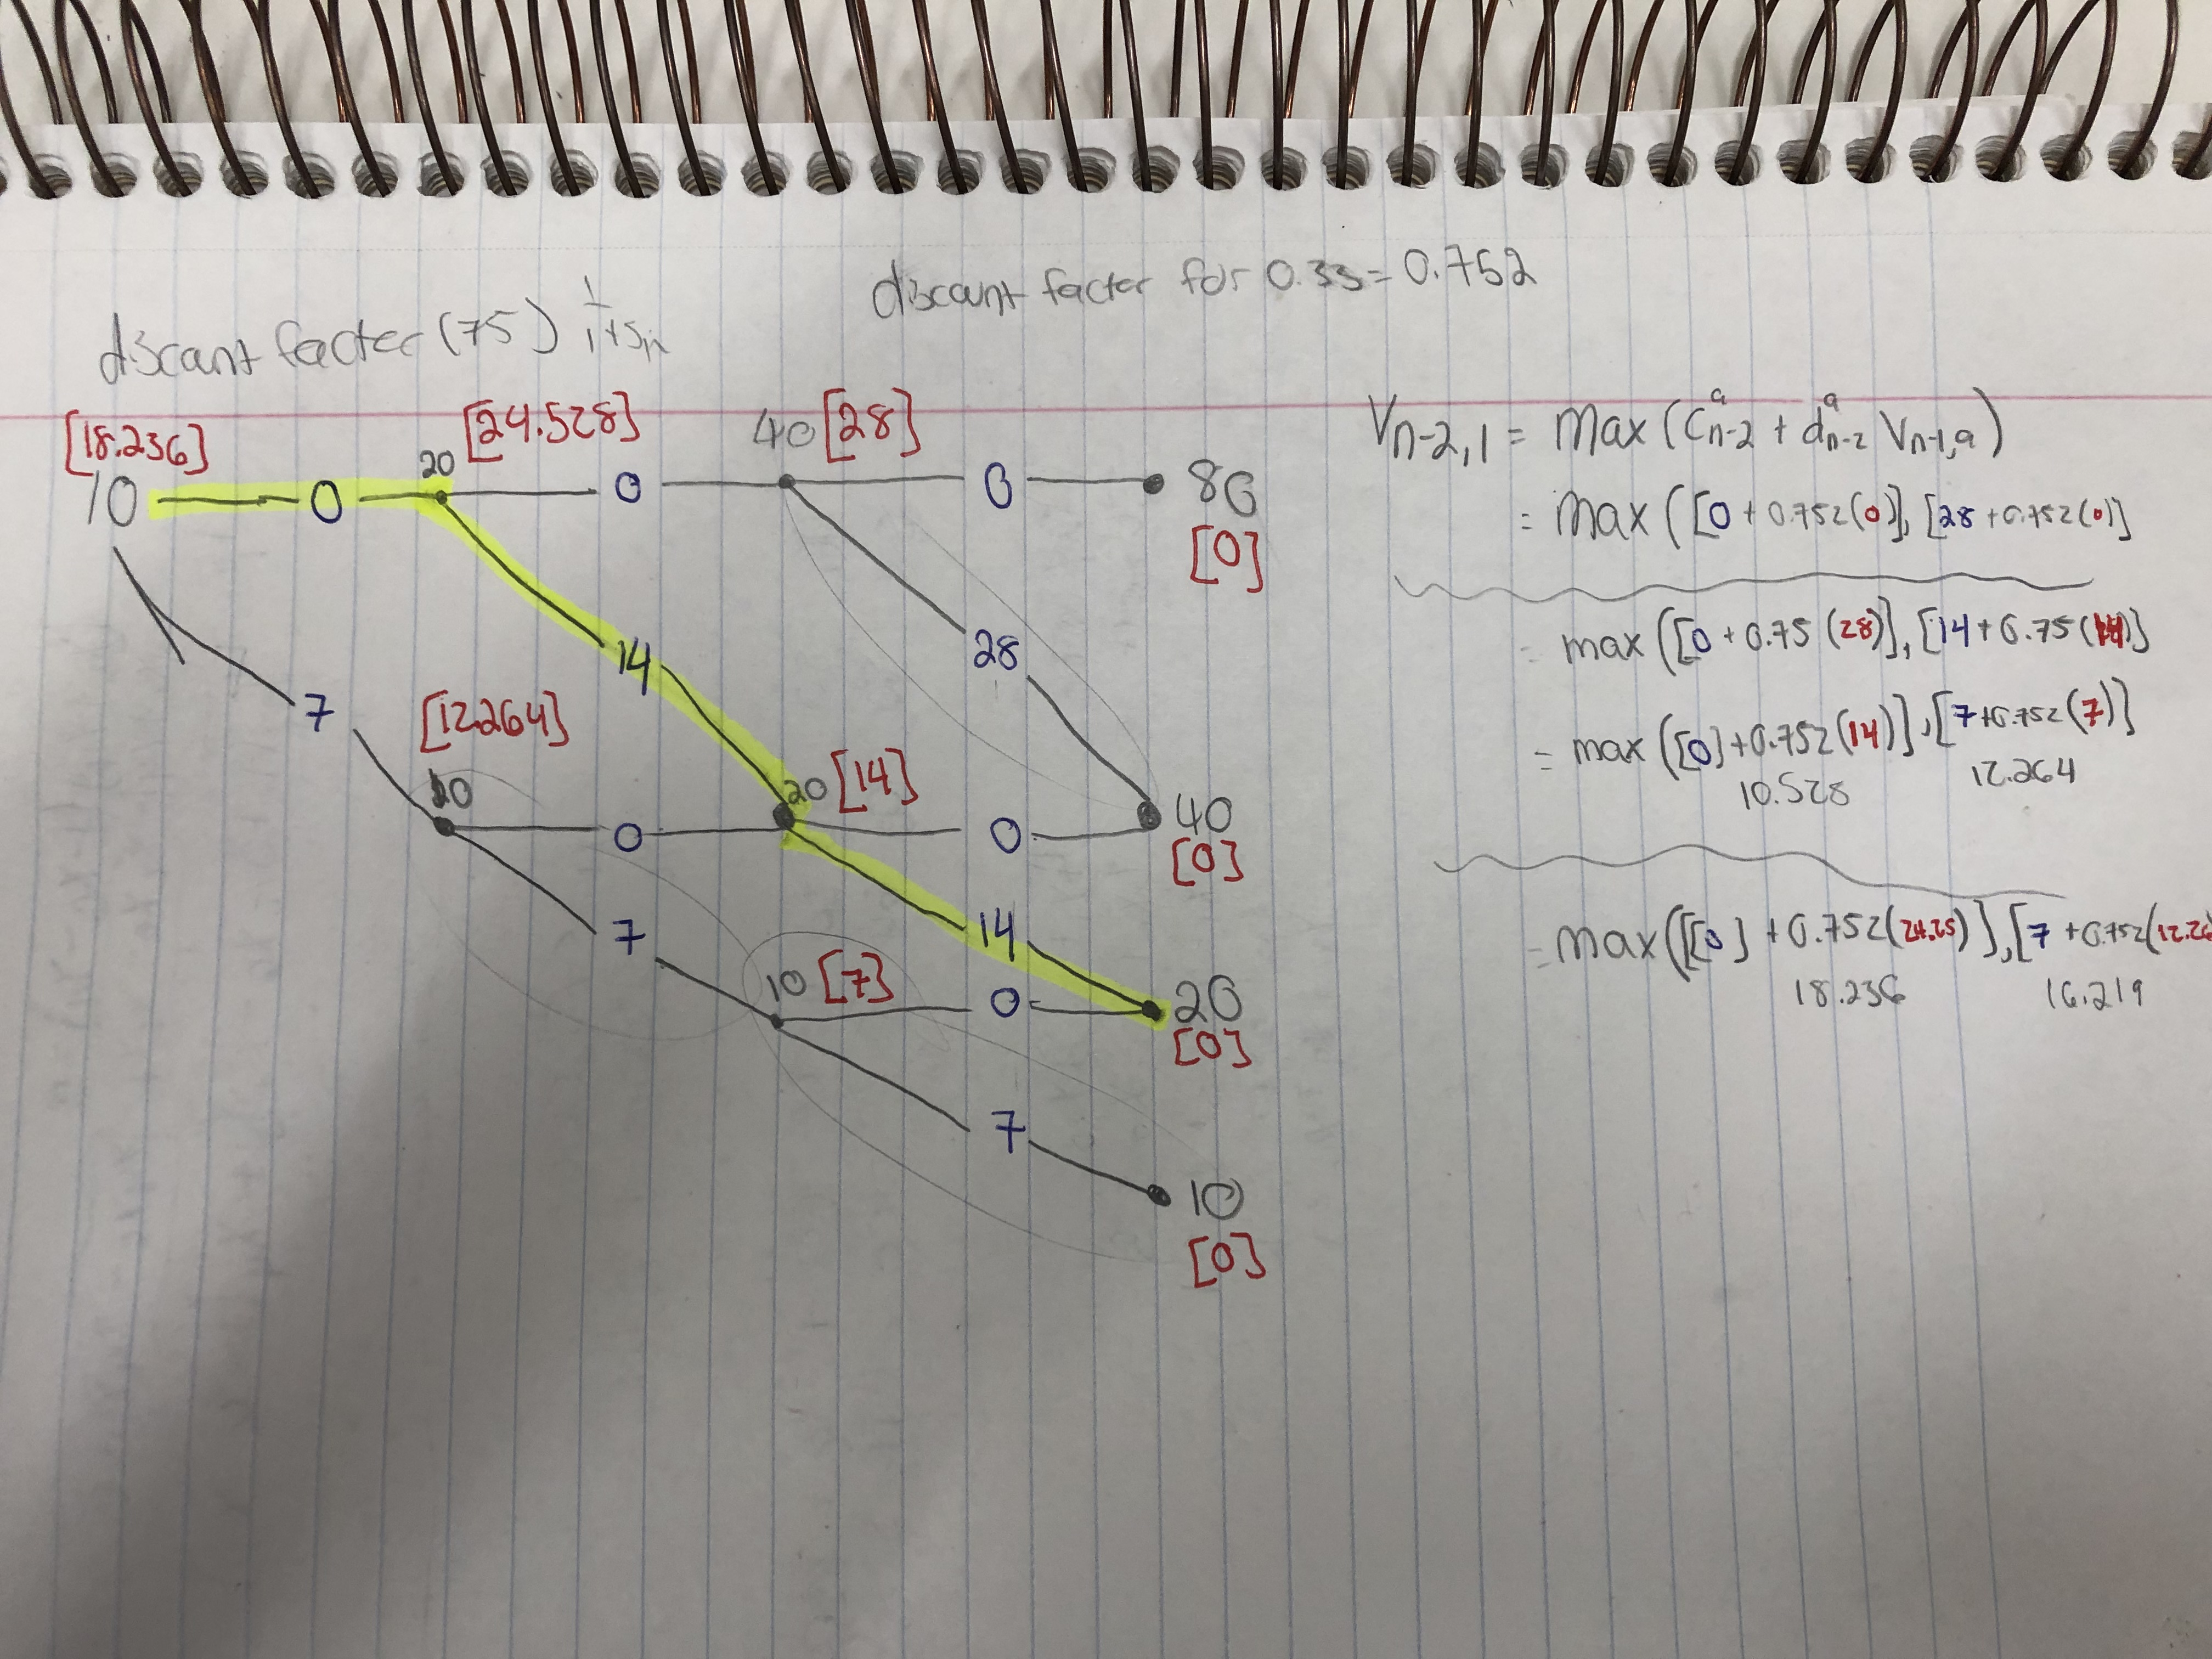
\includegraphics[width=0.59\linewidth]{mod4p7.jpg}
\end{center}

\end{problem}

\begin{problem}9. Three choices to pump oil: (a) not pump oil, (b) pump normally with operating cost 50,000 and you will pump out \%20 of what the reserves were at at the beginning, (c) enhanced pumping with 120,000 op cost and \%36 of your reserves. Price of oil is \$10/barrel and the interest rate is 10\% . 3 year period. Honestly, this art project took 45 minutes so I'm out of time and the rest of this seems like an easy time consuming exercise and I'm tired so I'll take the point. If I fail the class because of it so be it.  \\
\textbf{(a)} Show how to set up a trinomial lattice to represent the possible states of the oil reserves.\\
Well that was a pointless art project. The photo is below. \\
\begin{center}
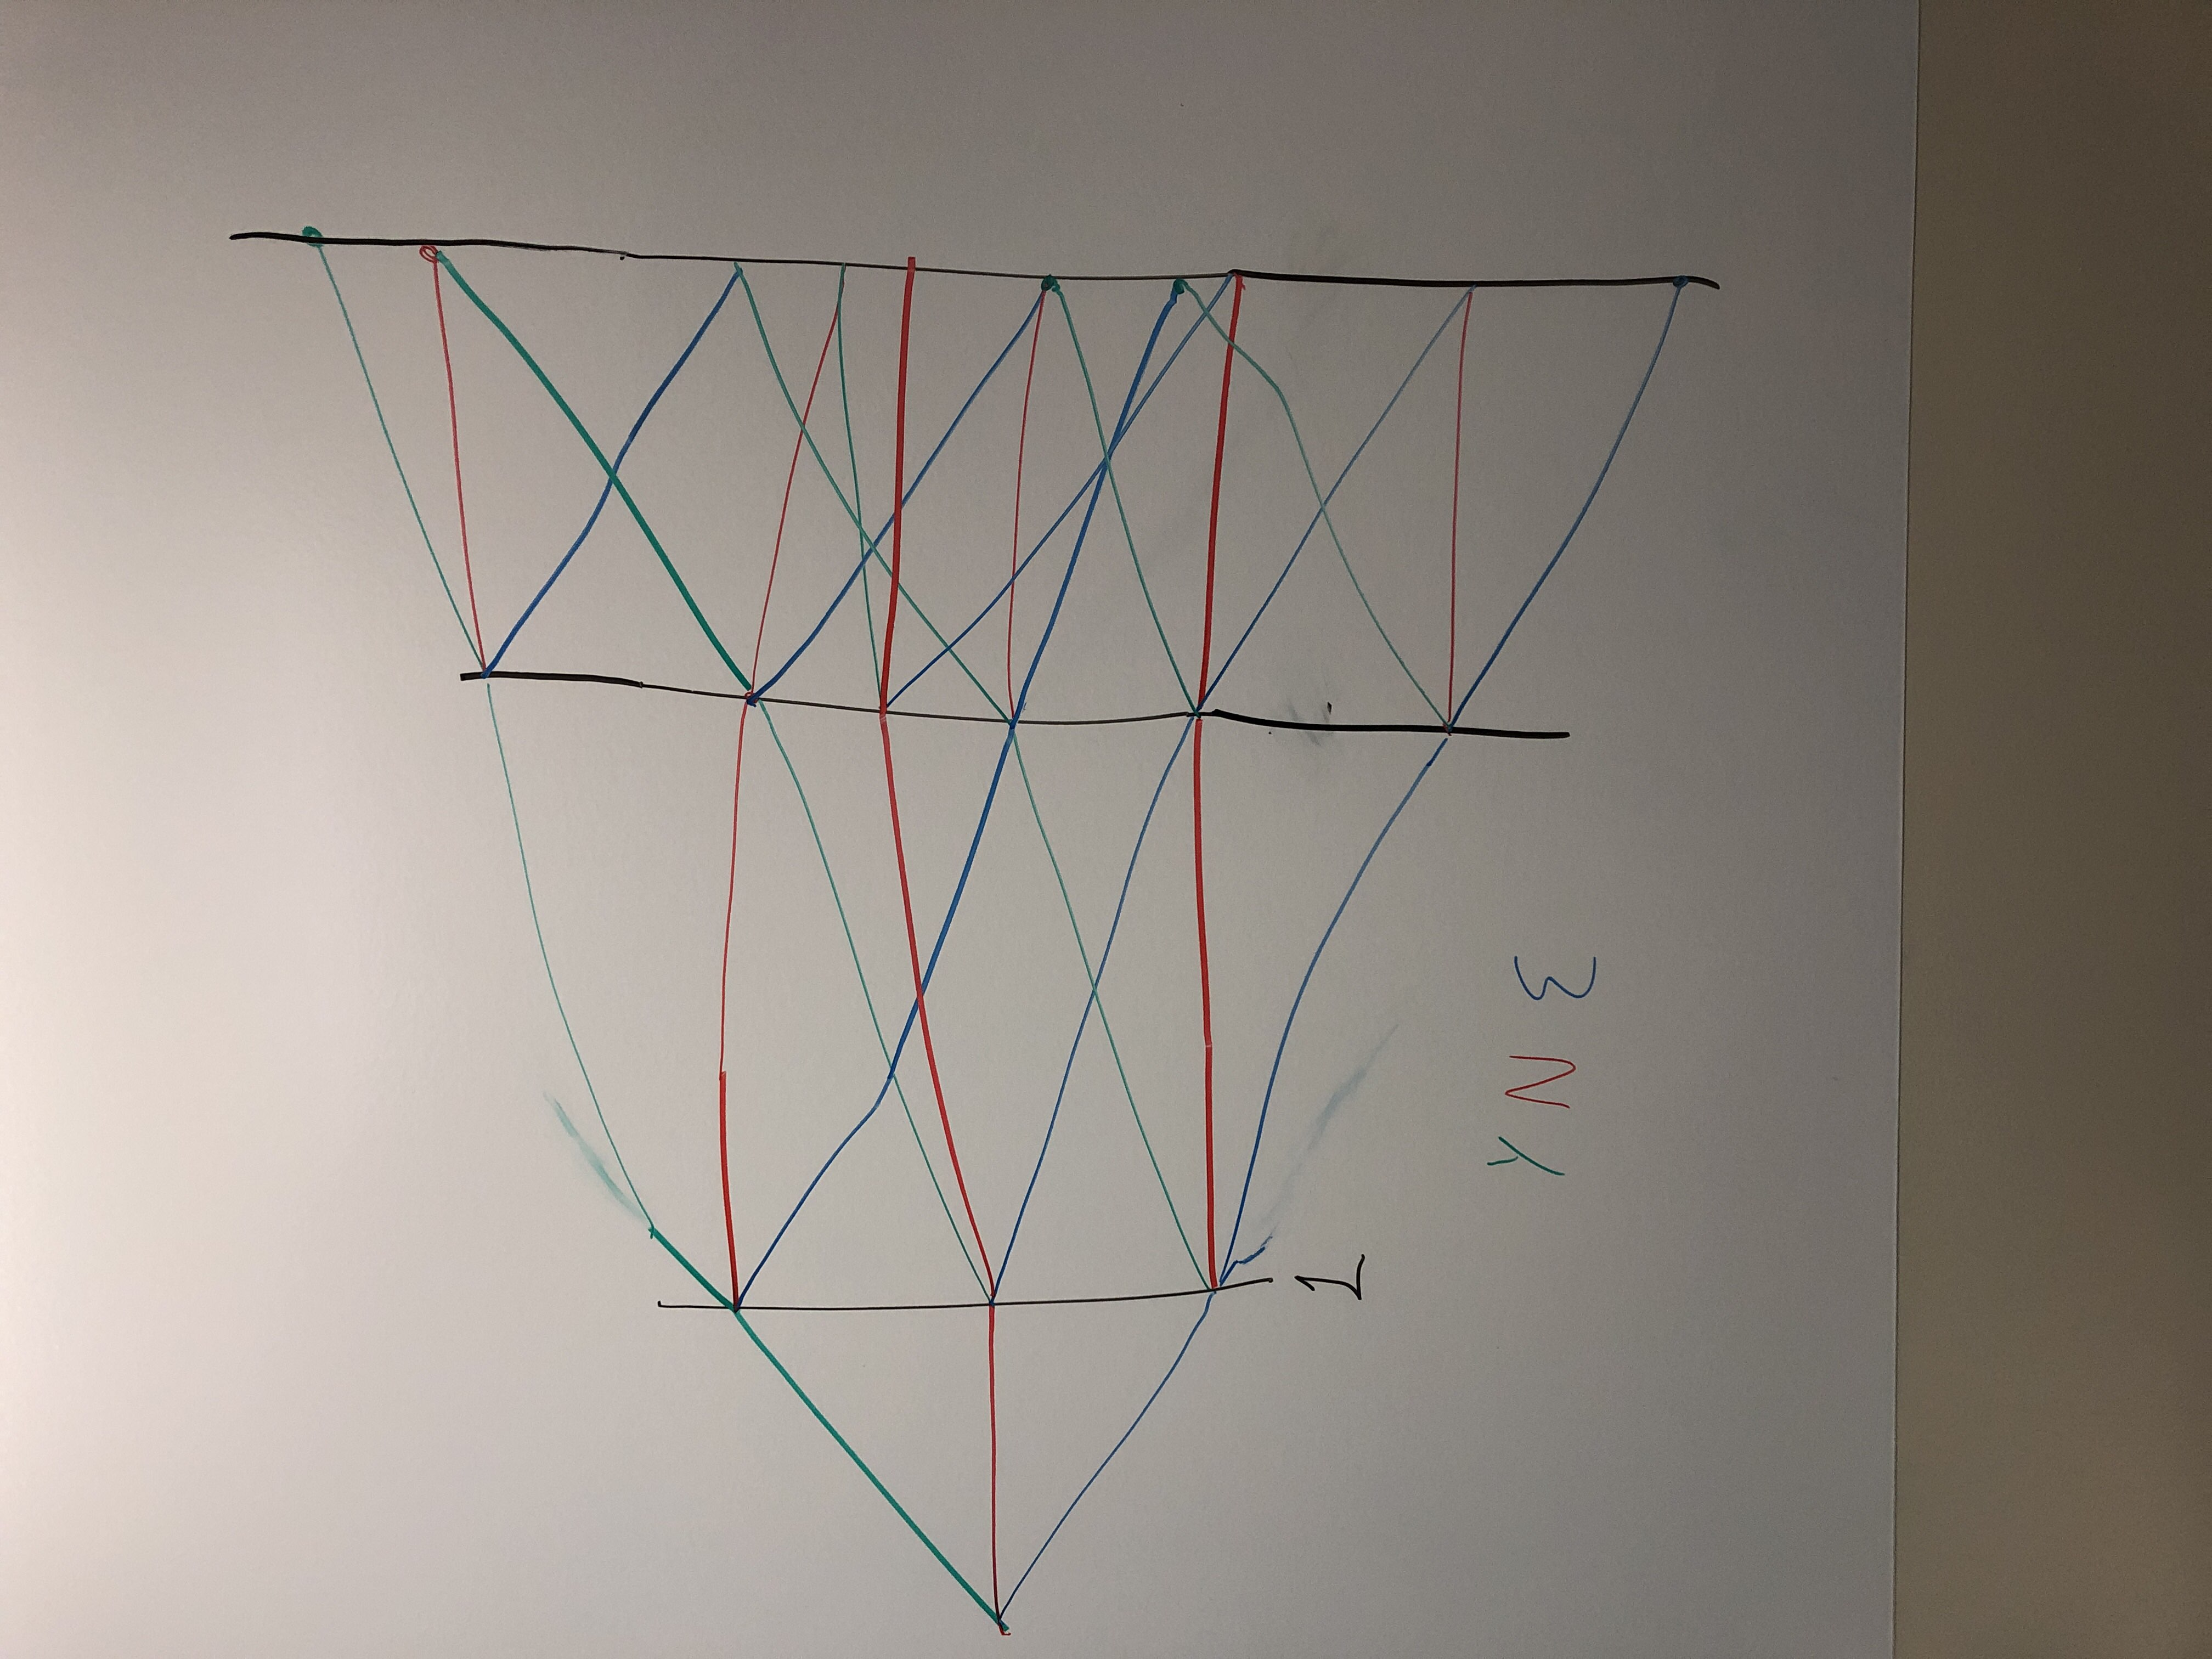
\includegraphics[width=0.59\linewidth]{mod4p9.jpg}
\end{center}

\textbf{b} What is the maximum present value of your profits, and what is the corresponding pumping strategy. 
\end{problem}


\begin{problem}{11} Show that for $ g<r $
\begin{align*}
\Sigma_{k=1}\frac{(1+g)^{k-1}}{(1+r)^k} &= \frac{1}{r-g} \\
&= S = \frac{1}{(1+r)}+\frac{S(1+g)}{1+r} &&\text{hint} \\
S*(1-\frac{(1+g)}{(1+r)}) &= \frac{1}{(1+r)} && \text{solve for S} \\ 
S*(\frac{r-g}{1+r}) &=  \frac{1}{(1+r)} \\ 
S &= \frac{1}{r-g} 
\end{align*}

\end{problem}


\end{document}



% Set the overall layout of the tree
\tikzstyle{level 1}=[level distance=3.5cm, sibling distance=3.5cm]
\tikzstyle{level 2}=[level distance=3.5cm, sibling distance=2cm]

% Define styles for bags and leafs
\tikzstyle{bag} = [text width=4em, text centered]
\tikzstyle{end} = [circle, minimum width=3pt,fill, inner sep=0pt]

\begin{tikzpicture}[grow=right, sloped]
\node[bag] {Bag 1 $4W, 3B$}
    child {
        node[bag] {Bag 2 $4W, 5B$}        
            child {
                node[end, label=right:
                    {$P(W_1\cap W_2)=\frac{4}{7}\cdot\frac{4}{9}$}] {}
                edge from parent
                node[above] {$W$}
                node[below]  {$\frac{4}{9}$}
            }
            child {
                node[end, label=right:
                    {$P(W_1\cap B_2)=\frac{4}{7}\cdot\frac{5}{9}$}] {}
                edge from parent
                node[above] {$B$}
                node[below]  {$\frac{5}{9}$}
            }
            edge from parent 
            node[above] {$W$}
            node[below]  {$\frac{4}{7}$}
    }
    child {
        node[bag] {Bag 2 $3W, 6B$}        
        child {
                node[end, label=right:
                    {$P(B_1\cap W_2)=\frac{3}{7}\cdot\frac{3}{9}$}] {}
                edge from parent
                node[above] {$B$}
                node[below]  {$\frac{3}{9}$}
            }
            child {
                node[end, label=right:
                    {$P(B_1\cap B_2)=\frac{3}{7}\cdot\frac{6}{9}$}] {}
                edge from parent
                node[above] {$W$}
                node[below]  {$\frac{6}{9}$}
            }
        edge from parent         
            node[above] {$B$}
            node[below]  {$\frac{3}{7}$}
    };
\end{tikzpicture}


\section{Definitions}
\underline{Def: Forward Rate Formulas} (pg 79). The implied forward rate between times $t_1$ and $t_2$ is the rate of interset between those times that is consistent with a given spot rate curve. For Yearly compounding, the forward rate is:  
\begin{align*}
f_{i,j} =& [\frac{(1+s_j)^j}{(1+s_i)^i}]^{1/(j-i)}-1 \\
 e^{s(t_2)t_2} =& e^{s(t_1)t_1}e^{f_{t_1,t_2}(t_2-t_1)}
\end{align*}

\underline{Discount Factor Relation} The discount facot between periods i and j is defined as $$ d_{i,j}=[\frac{1}{1+f_{i,j}}]^{j-i}$$ These factors satisfy the compounding rule: $d_{i,k}=d_{i,j}d_{j,k}$\\

\underline{Def. Derivative (Ross pg 223)} Let F be a real valued function defined on an open interval contained a point a. We say f is differentiable at a, or f has derivative at a if the limit $$ f'(a) = \lim_{x \to a} \frac{f(x)-f(a)}{x-a} $$




https://www.investopedia.com/university/advancedbond/bond-pricing.asp
https://quant.stackexchange.com/questions/22288/duration-of-perpetual-bond
http://people.stern.nyu.edu/gyang/foundations/sample-final-solutions.html
http://pages.stern.nyu.edu/~jcarpen0/courses/b403333/07convexh.pdf
https://web.stanford.edu/class/msande247s/2009/summer%2009%20week%205/Bond%20Formula%20Sheet.pdf


\underline{Def: Forward Rate Formulas} (pg 79). The implied forward rate between times $t_1$ and $t_2$ is the rate of interset between those times that is consistent with a given spot rate curve. For Yearly compounding, the forward rate is:  
\begin{align*}
f_{i,j} =& [\frac{(1+s_j)^j}{(1+s_i)^i}]^{1/(j-i)}-1 \\
 e^{s(t_2)t_2} =& e^{s(t_1)t_1}e^{f_{t_1,t_2}(t_2-t_1)}
\end{align*}

\underline{Discount Factor Relation} The discount facot between periods i and j is defined as $$ d_{i,j}=[\frac{1}{1+f_{i,j}}]^{j-i}$$ These factors satisfy the compounding rule: $d_{i,k}=d_{i,j}d_{j,k}$\\

\underline{Def. Derivative (Ross pg 223)} Let F be a real valued function defined on an open interval contained a point a. We say f is differentiable at a, or f has derivative at a if the limit $$ f'(a) = \lim_{x \to a} \frac{f(x)-f(a)}{x-a} $$



\begin{align*}
\text{Maximize  } & 4x_1 +5x_2 +3x_3 +4.3x_4 + x_5 + 1.5x_6 + 2.5x_7 + 0.3x_8 + x_9 + 2x_{10} \\
\text{Subject to } & 2x_1 + 3x_2 + 1.5x_3 + 2.2x_4 +0.5x_5 +15x_6 + 2.5x_7 +0.1x_8 + 0.6x_9 + x_{10} \leq 5 \\ 
& x_1 + x_2 + x_3 + x_4 \leq 1 \\
& x_5 + x_6 + x_7 \leq 1 \\
& x_8 + x_9 + x_{10} \leq 1 \\
\end{align*}